\documentclass[conference]{IEEEtran}

\usepackage{algorithmicx}
\usepackage[noend]{algpseudocode}
\usepackage[ruled,vlined]{algorithm2e}
\usepackage[]{array}

\algblock{ParFor}{EndParFor}
% customising the new block
\algnewcommand\algorithmicparfor{\textbf{ParFor}}
\algnewcommand\algorithmicpardo{\textbf{do}}
\algnewcommand\algorithmicendparfor{\textbf{end\ ParFor}}
\algrenewtext{ParFor}[1]{\algorithmicparfor\ #1\ \algorithmicpardo}
\algrenewtext{EndParFor}{\algorithmicendparfor}

% for numbered citations
\usepackage{cite}
% for figures based on pdfs
\usepackage[pdftex]{graphicx}
 
 % Ben's packages
\usepackage{pgfplots}
\pgfplotsset{compat=1.13}
\usepackage{times}
\usepackage{listings}
\graphicspath{ {images/} }


\begin{document}

\title{ParForPy: Loop Parallelism in Python}
\author{
\IEEEauthorblockA{Benjamin James Gaska}
\IEEEauthorblockA{Computer Science\\
University of Arizona\\
Tucson, Arizona\\
Email: bengaska@email.arizona.edu}}

\maketitle

\begin{abstract}

\end{abstract}

\section{Introduction}

%Paragraph 1, give problem. Scientific researchers like using high-level languages. We must work around their usage

The amount of data available to researchers has exploded in recent years,
whole fields are based in performing large dataset analysis.
Bioinformatics research involves searching through terrabytes of genetic data
to identify meaningful variations\cite{bolstad2003comparison}.
Social sciences are performing analysis of millions of tweets to detect political trends in lieu of traditional surveying methods. 
\cite{cody2016public}
Literary critics are building models of history of the novel through analysis of millions of books over hundreds of years\cite{moretti2005graphs}.
These users are searching for tools that enable them to quickly perform 
their analyses with minimal effort.
The programming language chosen, and the libraries available in the language, 
have the most direct impact upon the user's work.

Several high-level programming languages have become popular data analysis tasks, in particular SAS\cite{sas2004sas}, R\cite{team2000r}, and Python\cite{vanrossum2010python} have grown to dominate data analysis\cite{kdnuggetSurvey}.
Python in particular has grown to be one of the most popular general purpose programming languages, both in raw number of users\cite{kdnuggetSurvey} and rate 
of growth of its user base\cite{kdnuggetGrowthSurvey}.
This popularity comes despite the fact that Python is quite slow.
Runtime comparisons of bioinformatic algorithms
show Python to be, on average, an order of magnitude slower than 
compiled languages such as C/C++ and Java\cite{fourment2008comparison}.
Long runtimes can lead to Python becoming infeasible
for computationally expensive analyses.

Parallelism is a way to break through the processing bottleneck,
but Python has limited support for for parallelism.
The reference implementation of Python, CPython, has a 
Global Interpreter Lock (GIL) which ensures that only one thread 
has access to the interpreter at a given
time.\cite{beazley2010understanding}
This significantly impedes the usage of many types of parallelism.
If multiple threads are used, then all but one will block and wait for the
GIL to allow them to execute. 
This effectively kills the usefulness of threads as a means to improve
computation time.


Useful parallelism in Python is thus implemented as processes, which spawn
of their own data and interpreter and thus are free of restrictions of the GIL.
The multiprocessing module requires the user to implement parallelism 
either as a map or a task-worker queue. 
Both of these abstractions can differ significantly from the for-loop 
structure most familiar for Python users. 
This can require refactoring of the serial code, cause 
tangling of the parallel logic with the main algorithmic 
logic, and require usage models that can be unfamiliar with many users.
These issues create a significant impediment towards usage of parallelism in Python. 
Even when the problem matches well with the parallel tools available 
users can be discouraged from straying away from their serial 
implementation.

ParForPy is a way to overcome the runtime bottleneck by enabling
easy usage of parallelism in the language. 
Inspired by OpenMP's pragma-based model\cite{dagum1998openmp}, 
ParForPy allows users to specify which loops to parallelize. 
The specified loops are than
transformed to use the parallel tools available in Python. 
This is designed to minimally interfere with the underlying code logic.
This allows users to indicate loop-level parallelism without having to
significantly alter the serial code.


This paper presents the following contributions: 
\begin{enumerate}
    \item ParForPy a novel tool for transformation of serial Python code
    into parallel code,
    \item A survey of research scientist's programming habits, the
    bottlenecks they face and evidence that the ParForPy model is 
    preferred over other parallelization options in Python,
    \item Comparison of ParForPy performance in a variety of 
    common Python benchmarks and libraries,
    \item A case study evaluating the usage of ParForPy in
    a real-world planetary science code. 
\end{enumerate}

It is difficult to overcome the slowness of Python relative to
highly performant languages.
What is possible is making Python fast enough that it is not the 
bottleneck for the researcher's work.
This enables users to continue using Python, and the conveniences that 
brings, without excessively impeding the data pipelines that underpin 
modern scientific research.
In this way, we can enable researchers to perform their analysis
faster with less effort, freeing them to do more than they otherwise 
could.

%\section{Motivation}

%Scientific analysis is often limited by their data processing pipeline.
%Across topics as varied as cancer research \cite{danford2016analyzing} %and planetary science, (TODO: add arxiv paper)
%researchers are working with tools that are they are not able to make performant enough to satisfy their needs.
%This forces researchers to limit their work in some way, requiring coarser-grained analysis, analyzing less data than they would prefer,
%or even preventing some work from being done at all.
%Finding ways to circumvent these issues leads to improvement in
%many scientific endeavors.


%The Python Standard Library has two modules for parallelism:
%threading and multiprocessing, utilizing thread-based and 
%process-based parallelism respectively.

%This limits the performance improvements that can be achieved with
%threads.
%This necessitates working with heavyweight processes instead.

%The multiprocessing module requires the user to implement parallelism 
%either as a map or a task-worker queue. 
%Both of these abstractions can differ significantly from the for-loop 
%structure most familiar for Python users. 
%This can require significant refactoring of the serial code, cause 
%significant tangling of the parallel logic with the main algorithmic 
%logic, and require usage models that can be unfamiliar with many users.

%These issues create a significant impediment towards usage of parallelism in Python. 
%Even when the problem matches well with the parallel tools available 
%users can be discouraged from straying away from their serial 
%implementation.
%This is supported by survey data which shows that users tend to shy away %(TODO: Need to clarify some things, will extend further with discussion of programmer's tendency to avoid parallelism)




\section{Implementation}

The goal of ParForPy is to make the programmer responsible for identifying parallelism, 
allowing for an automatic transformation of the indicated for-loop. 
The ParForPy toolset is implemented as a single new ParFor object. 

The code's Abstract Syntax Tree (AST) is searched and the ParFor object
is associated with the loop immediately succeeding it.
Further analysis is done to identify what values created outside 
of the for-loop is needed for the computation inside the for-loop.
This information is combined with the information about which variables
are needed, as well as an optional reduction.
Tbe AST is then modfied to parallelize the loop, using the constructs available in the standard library. 
The transformed loop is exactly equivalent to the original serial construct, requiring no modification of any code outside of the 
parallelized loop to ensure correctness of the overall program.

Figure \ref{basicExample} shows a simple example of a singly-nested loop
which process the items in a collection and appends them to a list for 
further use somewhere later in the code.
Parallelization is indicated by the user explicitly by placing a ParFor 
object before the loop to be run in parallel.
The user passes into the ParFor constructor the variables they wish to have returned from the loop body.
Then, before runtime the Abstract Syntax Tree is transformed by ParForPy
to produce code that uses the built-in Python parallel constructs.


The only difference between the serial implementation and the ParForPy implementation is the introduction of the ParFor object.

\begin{figure}[t]
\begin{lstlisting}[frame=single]
ParFor(output=(x))
for i in collection:
    x.append(processXValue(i))
\end{lstlisting}
\caption{Simple example of parallelizing a for loop using Parfor. The loop builds up lists x by performing some computation on each value in the given collection of values.}
\label{basicExample}
\end{figure}

\section{Results}

The ParForPy implementation strives for simplicity, ease of use, and minimal difference between the serial and parallel code.
To this end, 40 benchmarks were chosen and an attempt was made to parallelize it using only the ParForPy parallelism model.

The benchmarks were sampled from a larger set of benchmarks made up of the following:
\begin{itemize}
   \item Python Performance Suite\cite{pyPerformance}, a collection of benchmarks for comparison of Python implementations
   \item Natural Language Toolkit (NLTK) \cite{bird_2016}, an 
   open-source codebase for natural language processing in Python.
   \item A selection of bioinformatics code use by scientific researchers
\end{itemize}
These were chosen because they represent a broad variety of code. 
This include implementation entirely in Python, and implementations 
that have a significant portion of its computation performed by calls to external C code.
CPython's native interfacing with C code makes the latter a particularly common usage case.
Further, Numpy, Scikit-Learn, and NLTK represent popular libraries for dataset analysis and scientific programming in Python.


ParForPy was evaluated on the code in two ways. First, we look at SLOC between
the ParForPy implementation, the serial implementation and a hand parallelized implementation.
The second takes the code the was able to be parallelized using our method and compares improvements in runtime of code.


\subsection{Source Lines of Code}

ParForPy works by taking a loop that is known to us and transforming the loop body
into a function call that can be used with the parallel tools that Python has available.
Because of this the manual implementation of parallelism for each code is not too 
significant of a change in SLOC.
The hand transformation involves factoring out loop bodies into a worker or function call.
This does not often translate to an overall huge change in the SLOC.
Figure \ref{slocchart} shows this clearly, with an approximately linear difference
between the serial and manually implemented versions.
This depends on the number of spots being parallelized, and so when the PESS implementation parallelizes in two places this about doubles the SLOC difference.
This is also true with the ParForPy version which consists of a single line of additional
code.

The more significant change is often to the structure of the code itself.
The programmer implements the parallelism either as a worker function or a function that
is mapped over the data.
It also means setting up a pool of workers, building a queue of tasks that the manager will give to workers, and joining the processes after the computation is completed.
This leads to the user having to implement non-trivial refactoring of their code. 
Further, this necessitates an extensive tangling of the requirements for parallelism with
the actual computation that is being specified. 

In many cases this can lead the user to avoiding using parallelism.
Even if parallelism is manually implemented the integration of parallel code and 
the cognitive overhead of the additional function names can negatively impact 
the ability to reason over their code.
There is also added difficulty for future users of the code, who have an extra mechanic 
that they must understand in conjunction with the actual computation occurring.
This does not map cleanly to a number like SLOC, but cannot be ignored for the burden
it can create on the user.


\begin{figure}[t]
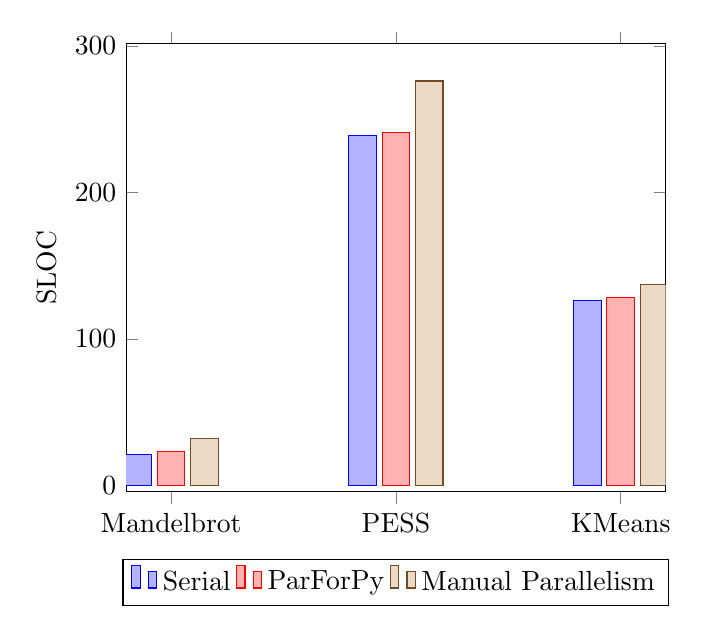
\begin{tikzpicture}
\centering
\begin{axis}[
    ybar,
    %enlargelimits=0.15,
    legend style={at={(0.5,-0.15)},
      anchor=north,legend columns=-1},
    ylabel={SLOC},
    symbolic x coords={Mandelbrot, PESS, KMeans},
    xtick=data,
    %nodes near coords,
    nodes near coords align={vertical},
    ]
\addplot 
	coordinates {(Mandelbrot,21)(PESS,239)(KMeans,126)};
\addplot 
	coordinates {(Mandelbrot,23)(PESS,241)(KMeans,128)};
\addplot
    coordinates {(Mandelbrot,32)(PESS,276)(KMeans,137)};
    
\legend{Serial,ParForPy, Manual Parallelism}
\end{axis}
\end{tikzpicture}
\caption{Source Lines of Code comparison against different implementations.
The ParForPy implementation stays very close to the serial implementation. While,
the manual implementation tends to be slightly higher.}
\label{slocchart}
\end{figure}

\subsection{Mandelbrot Set}

Computing the Mandelbrot Set is a common introductory programming task for parallel
computing.
Each row of the final image can be computed separately from every other,
making it a simple to parallelize task, with low concern for workload imbalance.
We choose to use this as a baseline and proof of concept for the ParForPy model.

Testing was done by generating a 1,000 x 1,000 pixel image, where each pixel was drawn by
calculating the Mandelbrot sequence out to 10,000 iterations.
Figure \ref{SpeedUpResults} shows the speed-up as the number of processes used increases.
As the number of processes increases to 10 the results are as expected. 
We see near 1-to-1 gains of speed-up to number of processes.
After 10 though the gains fall off almost completely.

This is important to note. 
There is not an obvious hardware limitation leading to this, there are 12 cores available for use and so we should expect gains up until that point. 
We will see with the other experiments done that extreme fall-off in improvements occurs 
at 10 processes as well.
This gives possible insight into a further restriction of the Python multiprocessing toolset. 
That some aspect of the overhead beings to spike at this point, limiting gains beyond this point.
This seems to effectively limit our possible scaling in a Python implementation.

\subsection{Protein Folding}

Protein Empirical Structure Space (PESS) is a codebase for performing protein
threading and classification\cite{middleton2016complete}. 
It is written in Python, making calls to an external C library for the
most computationally expensive parts of the process.
This mixing of Python and C code is common in scientific computing, due to CPython's 
ability to natively interop with C\cite{pythonCInterop}.

Data is read in as a series of Fasta strings, a file format for representing 
nucleotide sequences as character string.
Each of these can be evaluated independently of each other.
Each nucleotide sequence takes between 5 and 10 minutes to process, with
the largest portion of time taking place in the call to the external C code.
This minimizes the amount of time spent managing the subprocesses, and maximizes
the amount of time that each process can spend evaluation the sequence without 
any communication to the process manager.
This matches well with the restraints of Python multiprocessing.

Testing was done on a set of 20 nucleotide sequences.
In figure \ref{SpeedUpResults} we can see the Speed-Up as the number of processes
used increases.
The parallelism scales well to increases in the number of processes used, with
the speed-up improving at a close to 1-to-1 rate.
Noise is seen in the scaling, which is a result of the varying analysis time
needed for different nucleotide sequences. 
This is an underlying feature of the data that cannot be known until after performing 
analysis.
Because the major aspects of the computation are done in a pre-compiled C library further
optimization of this imbalance is not possible without fundamentally changing PESS.
In general, this case of parallelizing a large amount of independent tasks seems well fit to the ParForPy model.

\begin{figure}[t]
\centering
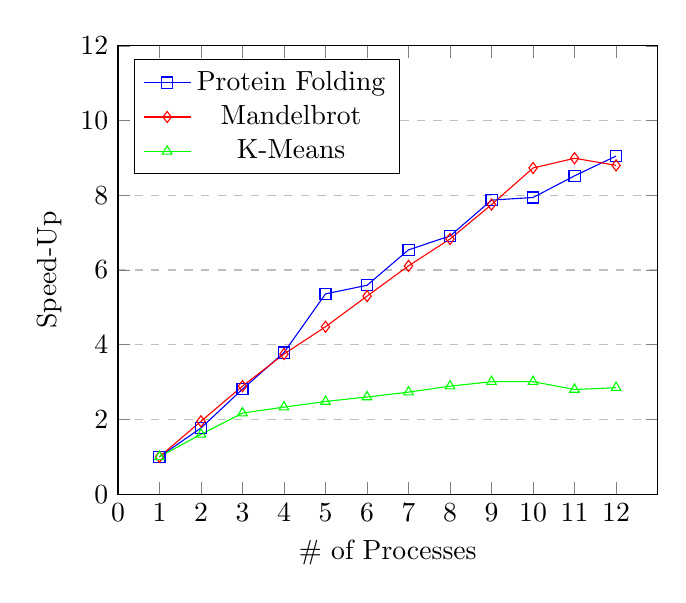
\begin{tikzpicture}
\begin{axis}[
    xlabel = {\# of Processes},
    ylabel = {Speed-Up},
    xmin=0, xmax=13,
    ymin=0, ymax=12,
    xtick={0,1,2,3,4,5,6,7,8,9,10,11,12},
    legend pos=north west,
    ymajorgrids=true,
    grid style=dashed,
]
 
\addplot[
    color=blue,
    mark=square,
    ]
    coordinates {
    (1,1)(2,1.77)(3,2.81)(4,3.79)(5,5.36)(6,5.59)(7,6.539)
    (8,6.91)(9,7.87)(10,7.94)(11, 8.52)(12,9.05)
    };
    
    \addplot[
    color=red,
    mark=diamond
    ]
    coordinates {
    (1,1)(2,1.95)(3,2.89)(4,3.75)(5,4.48)(6,5.30)(7,6.11)(8,6.83)(9,7.75)(10,8.73)(11,8.99)(12,8.80)
   };
   
    \addplot[
     color=green,
     mark=triangle
     ]
     coordinates {
     (1,1)(2,1.6)(3,2.17)(4,2.33)(5,2.48)(6,2.6)(7,2.73)(8,2.89)(9,3.01)(10,3.01)(11,2.8)(12,2.85)    
     };
     \legend{Protein Folding, Mandelbrot, K-Means}
     
\end{axis}
\end{tikzpicture}
\caption{Comparison of Speed-Up for each of the experiments discussed.}
\label{SpeedUpResults}
\end{figure}


\subsection{Naive Bayes Classification}

Naive Bayes is a supervised machine learning model, based on Bayes Theorem. 
In supervised learning,
the programmer trains the model by representing each data point as a series of features.
The model then associates different features to different degrees with the label given for 
each data point.

Specifically, Naive Bayes counts up the occurrences of each feature associated with a each label. 
Then, when a new data point is to be classified the model uses the data it has seen before and applies Bayes' Rule:

\begin{equation}
    \Pr(A|B)=\frac{\Pr(B|A)\Pr(A)}{\Pr(B)}
\end{equation}

The Naive in Naive Bayes refers to the simplifying assumption that the different features
are independent of one another. 
For instance, if we had a sentence "the boy went home", the occurrence of "the" would 
have no impact on the probability of "boy" appearing next. 
This simplifying assumption allows us to then simply count up the individual occurrences
of each feature with each label and use this to build a probability of each label occuring
for each label.


NOT DONE

%There can be significant noise and overlap between the features of different labels. 
%The goal is to uncover enough correlation during learning that we can correctly 
%label previously unseen data.




This and the following machine learning algorithms were training used the 20 Newsgroup corpus\cite{20Newsgroup}.
This corpus is a collection of postings to 20 different newsgroup in the early to late
90s.
It is a common corpus, that is used for a variety of supervised and unsupervised learning
training.
For Naive Bayes the associated newsgroup was used as the label, and the task becomes to
correctly identify which newsgroup a given text came from.


\subsection{Perceptron}

PLACEHOLDER

\subsection{K-Means Clustering}

K-Means\cite{forgy1965cluster} is an algorithm for unsupervised machine learning. 
Unlike the previous Naive Bayes model, no prior labeling of the data is required.
Instead, unsupervised learning attempts to derive natural clusters from 
the data without any external label.
This saves users the task of having to hand-label all training data 
beforehand, allowing for application on much larger datasets than would 
otherwise be possible.

The algorithm consists of taking data that is represented as a series of vectors.
The user chooses ahead of time a number of clusters they wish to be computed, in
our testing case 20 clusters were chosen. 
Then, a number of data points equal to the number of clusters are chosen at random,
these are the initial configuration of centroids for the algorithm.
Now for each iteration of the algorithm each data point is clustered with its
closest centroid.
Once all data is associated with a centroid, new centroids are created which are the
average of all of the vectors in that cluster.
This process is then repeated until the data converges and no data points change clusters
between iterations.
It is simple to understand and to implement and so has remained  a popular clustering technique.

With K-Means the number of iterations that occur cannot be known ahead of time, it runs
until convergence occurs. 
Each iteration directly depends on the results of the previous iteration and so we cannot parallelize over this dimension of the iteration space.
Parallelization instead occurs over the update portion of the algorithm, when each data 
point is compared against each centroid and sorted into a cluster.
At this point, each centroid is fixed and each data point can be assigned to a cluster
independently of one another.

Testing was done using the Newsgroup20 corpus, and each document was represented as a 
vector of word counts.
The task then becomes to see if the unsupervised clusters can group documents
along the original newsgroup sources.
Figure \ref{SpeedUpResults} shows speed-up as number of processes was increased.
Compared to the Mandlebrot and Protein Folding codes K-means sees less improvement from parallelization.
With those two we have a fair amount of computation that is divided among the subprocesses once.
This minimizes the cost of overhead, as the communication only needs to be done
once to divide work and once to collect results, the time spent on computation
is significantly greater than the time spent doing this communications.

With K-Means we must make a parallel call on each iteration, and each process is doing 
a relatively small amount of computation, as it simply compares each data point
to each of the 20 centroids and chooses the closest. 
Gains occur but they are more heavily impacted by the communication costs required by 
this action.
This particularly impacts scaling, as communication across more processes adds more and
more overhead dampening the possible runtime improvements as the number of processes used
increases.
In this case we ultimately see the improvment falling off hard, gaining only 3.01x speed-up at 10 processes. 
It begins to fall off thereafter as communication costs begin to overcome possible gains.

\section{Related Work}

PLACEHOLDER 
%PyMP\cite{pymp} is a library for Python that allows parallel iterators 
%in Unix environments. 
%It relies on making direct calls to the fork() system  k
%call, and is not compatible with non-Unix environments. t
%Further, it does not support reductions and can require 
%non-trivial rewrites of the serial code to fit within the model.

%Danford and Welch\cite{danford2016analyzing} takes a pre-existing


\section{Conclusions}

PLACEHOLDER



\bibliographystyle{IEEEtran}
\bibliography{Thesis}
\end{document}
